\documentclass{standalone}

% math and formulas
\usepackage{amsmath}
\usepackage{amsfonts}
\usepackage{amssymb}
\usepackage[amssymb]{SIunits}
\usepackage{mathtools}
\usepackage{esvect} % for vector typesetting
\usepackage{bm} % for matrix typesetting
\usepackage{xfrac}

\usepackage{environ}


\newcommand{\mat}[1]{\mathbf{#1}}
\let\oldvec\vec
\renewcommand{\vec}[1]{\mathbf{#1}}
\newcommand{\ten}[1]{\mathbf{#1}}

%transpose
\newcommand{\trans}[1]{#1^\mathrm{T}}

\newcommand{\keyword}[1]{\textbf{#1}}


% \renewcommand{\vec}[1]{\vv{#1}}

% ----------- TIKZ ---------------


\NewEnviron{defbox}[1]
{
  \centering

  \tikzstyle{mybox} = [draw=red, fill=blue!40!bgcolor, very thick, rectangle, rounded corners, inner sep=10pt, inner ysep=20pt]
  \tikzstyle{fancytitle} = [fill=red, text=white]
  \begin{tikzpicture}
    \node [mybox] (box) {%
      \begin{minipage}{1.0\textwidth}
        \BODY
      \end{minipage}
    };
    \node [right,inner xsep=1em,fill=red!75, text=white,outer sep=0pt,text height=2ex,text depth=.5ex] (title)
    at ([shift={(-1em,0pt)}]box.north west) {#1};
    \fill[red!50!black] (title.north east) -- +(-1em,1em) -- +(-1em,0) -- cycle;
    \fill[red!50!black] (title.south west) -- +(1em,-1em) -- +(1em,0) -- cycle;

  \end{tikzpicture}
}

\NewEnviron{infobox}[1]
{

  \tikzstyle{mybox} = [draw=blue, fill=green!20!black, very thick, rectangle, rounded corners, inner sep=10pt, inner ysep=20pt]
  \tikzstyle{fancytitle} = [fill=blue, text=white]
  \begin{tikzpicture}
    \node [mybox] (box) {%
      \begin{minipage}{1.0\textwidth}
        \BODY
      \end{minipage}

    };
    \node[fancytitle,right=10pt] at (box.north west) {#1};

  \end{tikzpicture}
}



%%% Local Variables:
%%% mode: latex
%%% TeX-master: "../main"
%%% End:


\usepackage{xcolor}
\usepackage{tikz}
\usetikzlibrary{external,3d,matrix,chains,positioning,calc,intersections,shapes,arrows,fadings,patterns,arrows.meta}
%\tikzexternalize
\usepackage{tikzpagenodes}
\usepackage{pgfplots}
\pgfplotsset{compat=1.16}

\begin{document}
\colorlet{pagecolor}{white}
\colorlet{textcolor}{black}

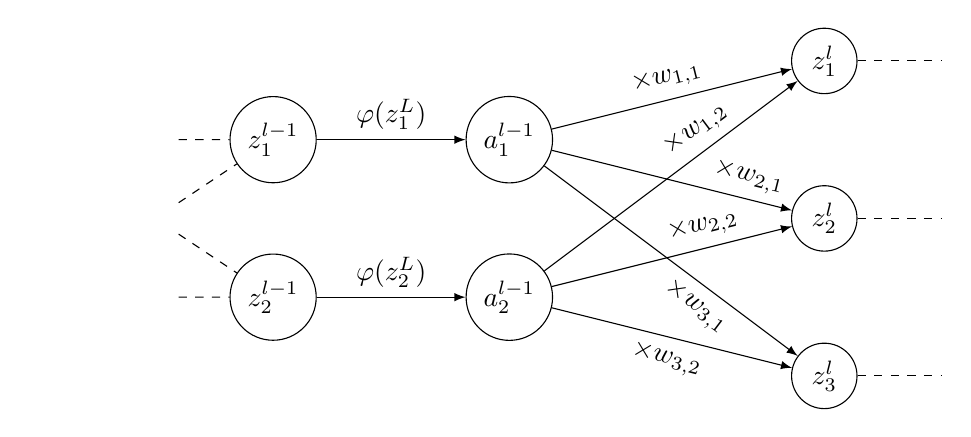
\begin{tikzpicture}[>=latex]
  \path (0,1) node [circle,draw](z1-){$z_1^{l-1}$};
  \path (0,-1) node [circle,draw](z2-){$z_2^{l-1}$};
  \path (3,1) node [circle,draw](a1-){$a_1^{l-1}$};
  \path (3,-1) node [circle,draw](a2-){$a_2^{l-1}$};
  \path (7,2) node [circle,draw](z1){$z_1^l$};
  \path (7,0) node [circle,draw](z2){$z_2^l$};
  \path (7,-2) node [circle,draw](z3){$z_3^l$};

  \draw[->] (z1-) -- node[above,sloped]{$\varphi(z_1^L)$} (a1-);
  \draw[->] (z2-) -- node[above,sloped]{$\varphi(z_2^L)$} (a2-);

  \draw[->] (a1-) -- node[sloped,above]{$\times w_{1,1}$} (z1);
  \draw[->] (a1-) -- node[sloped,above,pos=0.8]{$\times w_{2,1}$} (z2);
  \draw[->] (a1-) -- node[sloped,below,pos=0.65]{$\times w_{3,1}$} (z3);
  \draw[->] (a2-) -- node[sloped,above,pos=0.65]{$\times w_{1,2}$} (z1);
  \draw[->] (a2-) -- node[sloped,above,pos=0.65]{$\times w_{2,2}$} (z2);
  \draw[->] (a2-) -- node[sloped,below]{$\times w_{3,2}$} (z3);

  % endings
  \node (beg1) at (-3,1) {};
  \node (beg2) at (-3,-1) {};
  \draw[dashed] ($(beg1)!0.6!(z1-)$) -- (z1-);
  \draw[dashed] ($(beg1)!0.6!(z2-)$) -- (z2-);
  \draw[dashed] ($(beg2)!0.6!(z1-)$) -- (z1-);
  \draw[dashed] ($(beg2)!0.6!(z2-)$) -- (z2-);

  \draw[dashed] (z1) -- ++(1.5,0);
  \draw[dashed] (z2) -- ++(1.5,0);
  \draw[dashed] (z3) -- ++(1.5,0);

\end{tikzpicture}
%%% Local Variables:
%%% mode: latex
%%% TeX-master: "../figs"
%%% End:


\end{document}

%%% Local Variables:
%%% TeX-command-extra-options: "--shell-escape"
%%% TeX-master: "./figs"
%%% End: